\begin{evenBlock}{Gate Dribbling (10 min)}
Set up 3 gates in a zig-zag pattern about 6 to 10 yards apart.  The gates should be about a yard wide or less depending on dribbling skill of the group.  Players start a the end line and dribble through the gates as fast as possible.  Use the same technique as the previous drill.
\end{evenBlock}

\begin{oddBlock}{Gate Dribbling (10 min)}

\begin{minipage}[t]{\linewidth}
    \centering
    
    \begin{minipage}{.3\linewidth} % Left column and width
        %\begin{figure}
            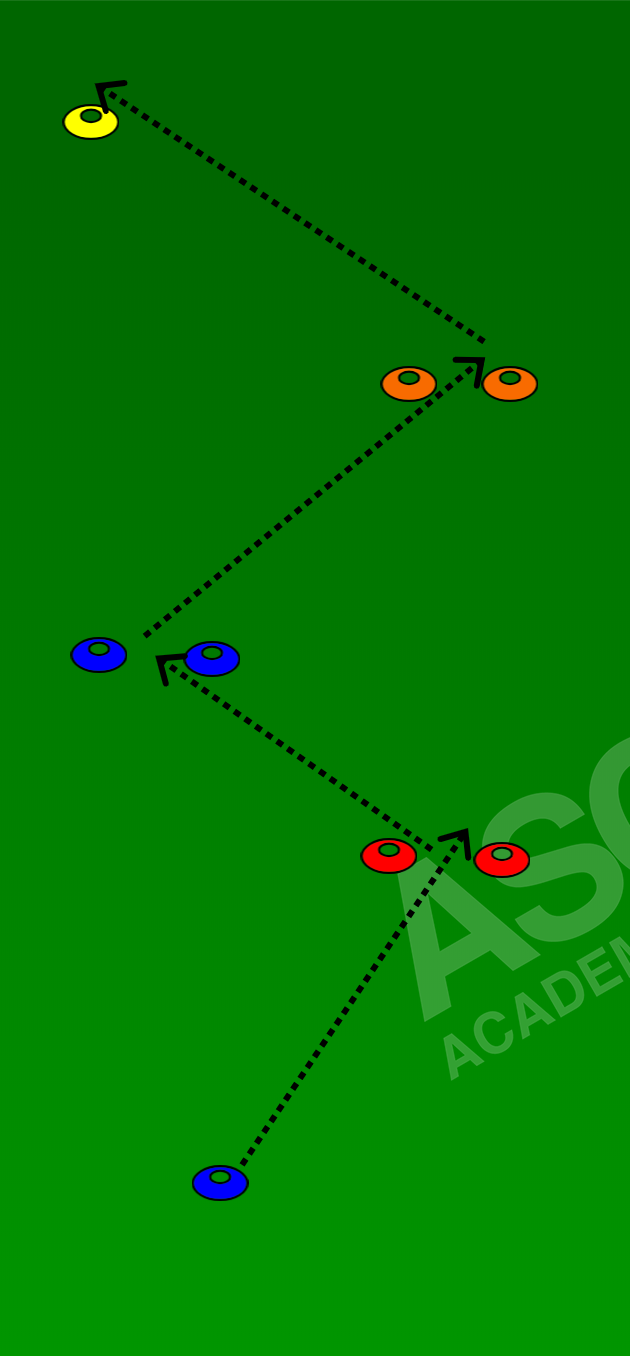
\includegraphics[width=.6\textwidth]{../img/Trimmed/Gate_Dribbling}
        %    \caption{Drill: 4 Person Passing}
        %\end{figure}
    \end{minipage}
    \hspace{0.05\linewidth}
    \begin{minipage}{.6\linewidth} % Left column and width
        \textbf{Drill Description:}
        The object is to dribble at full speed through 3 narrow gates set in a zig-zag pattern about 6 to 10 yards apart.  The gates should be about a yard wide or less depending on dribbling skill of the group.  Once they explode past the yellow cone, they jog back to the end of the line.  Use speed dribbling technique.
        \begin{enumerate}
        \setlength{\itemsep}{0pt}
        \setlength{\parskip}{0pt}
        \setlength{\parsep}{0pt}
        \item Players start at blue gate
        \item Then dribble the ball through the gates.
        \item Once they dribble through the orange gate they explode past the yellow cone.
        \item Then jog back to the end of the line.
        \end{enumerate}

        \textbf{Coaching Points:}
        \begin{itemize}
        \setlength{\itemsep}{0pt}
        \setlength{\parskip}{0pt}
        \setlength{\parsep}{0pt}
        \item When first starting, it will help to focus on proper technique over speed.  Increase the speed as the their technique improves.
        \item Technique uses top outside of the foot, toe down, pushing the ball forward 2 or 3 steps.
        \item Set width of of the gate based on skill.
        \end{itemize}

    \end{minipage}
\end{minipage}

\end{oddBlock}